\chapter{TINJAUAN PUSTAKA}

\section{Sistem Visi Komputer Tertanam (\textit{Embedded Computer Vision})}
Sistem visi komputer tertanam (\textit{embedded computer vision}) merupakan bidang interdisipliner yang menggabungkan perangkat keras sistem tertanam (\textit{embedded system}) dengan algoritma visi komputer untuk mengeksekusi tugas pemrosesan citra secara mandiri \cite{szeliski2022}. Berbeda dengan arsitektur komputasi awan yang memproses data visual di peladen jarak jauh, sistem tertanam dirancang untuk melakukan inferensi langsung di lokasi tempat data diakuisisi. Pendekatan ini sangat krusial dalam pengendalian robotika \textit{real-time}, karena menghilangkan dependensi terhadap konektivitas jaringan eksternal dan secara dramatis memangkas waktu tunda transmisi (\textit{transmission delay}) \cite{li2018}.

Pengaplikasian visi tertanam pada robotika modern juga memberikan keuntungan signifikan dari segi desain mekanis. Karena seluruh beban komputasi visi diselesaikan oleh \textit{microcomputer} yang berdimensi kecil, sistem ini secara substansial mengurangi beban muatan (\textit{payload}) dan konsumsi daya (\textit{power consumption}) dibandingkan dengan menggunakan \textit{Personal Computer} (PC) konvensional \cite{shi2016}. Hal ini memungkinkan perancangan lengan robot manipulator yang lebih ringkas, mandiri, dan fleksibel untuk diintegrasikan ke dalam berbagai lingkungan kerja spasial tanpa memerlukan infrastruktur jaringan yang kompleks. Implementasi antarmuka sistem visi komputer tertanam pada stasiun kerja kendali Dobot Magician ditunjukkan pada Gambar \ref{fig:antarmuka_dobot}.

\begin{figure}[htbp]
    \centering
    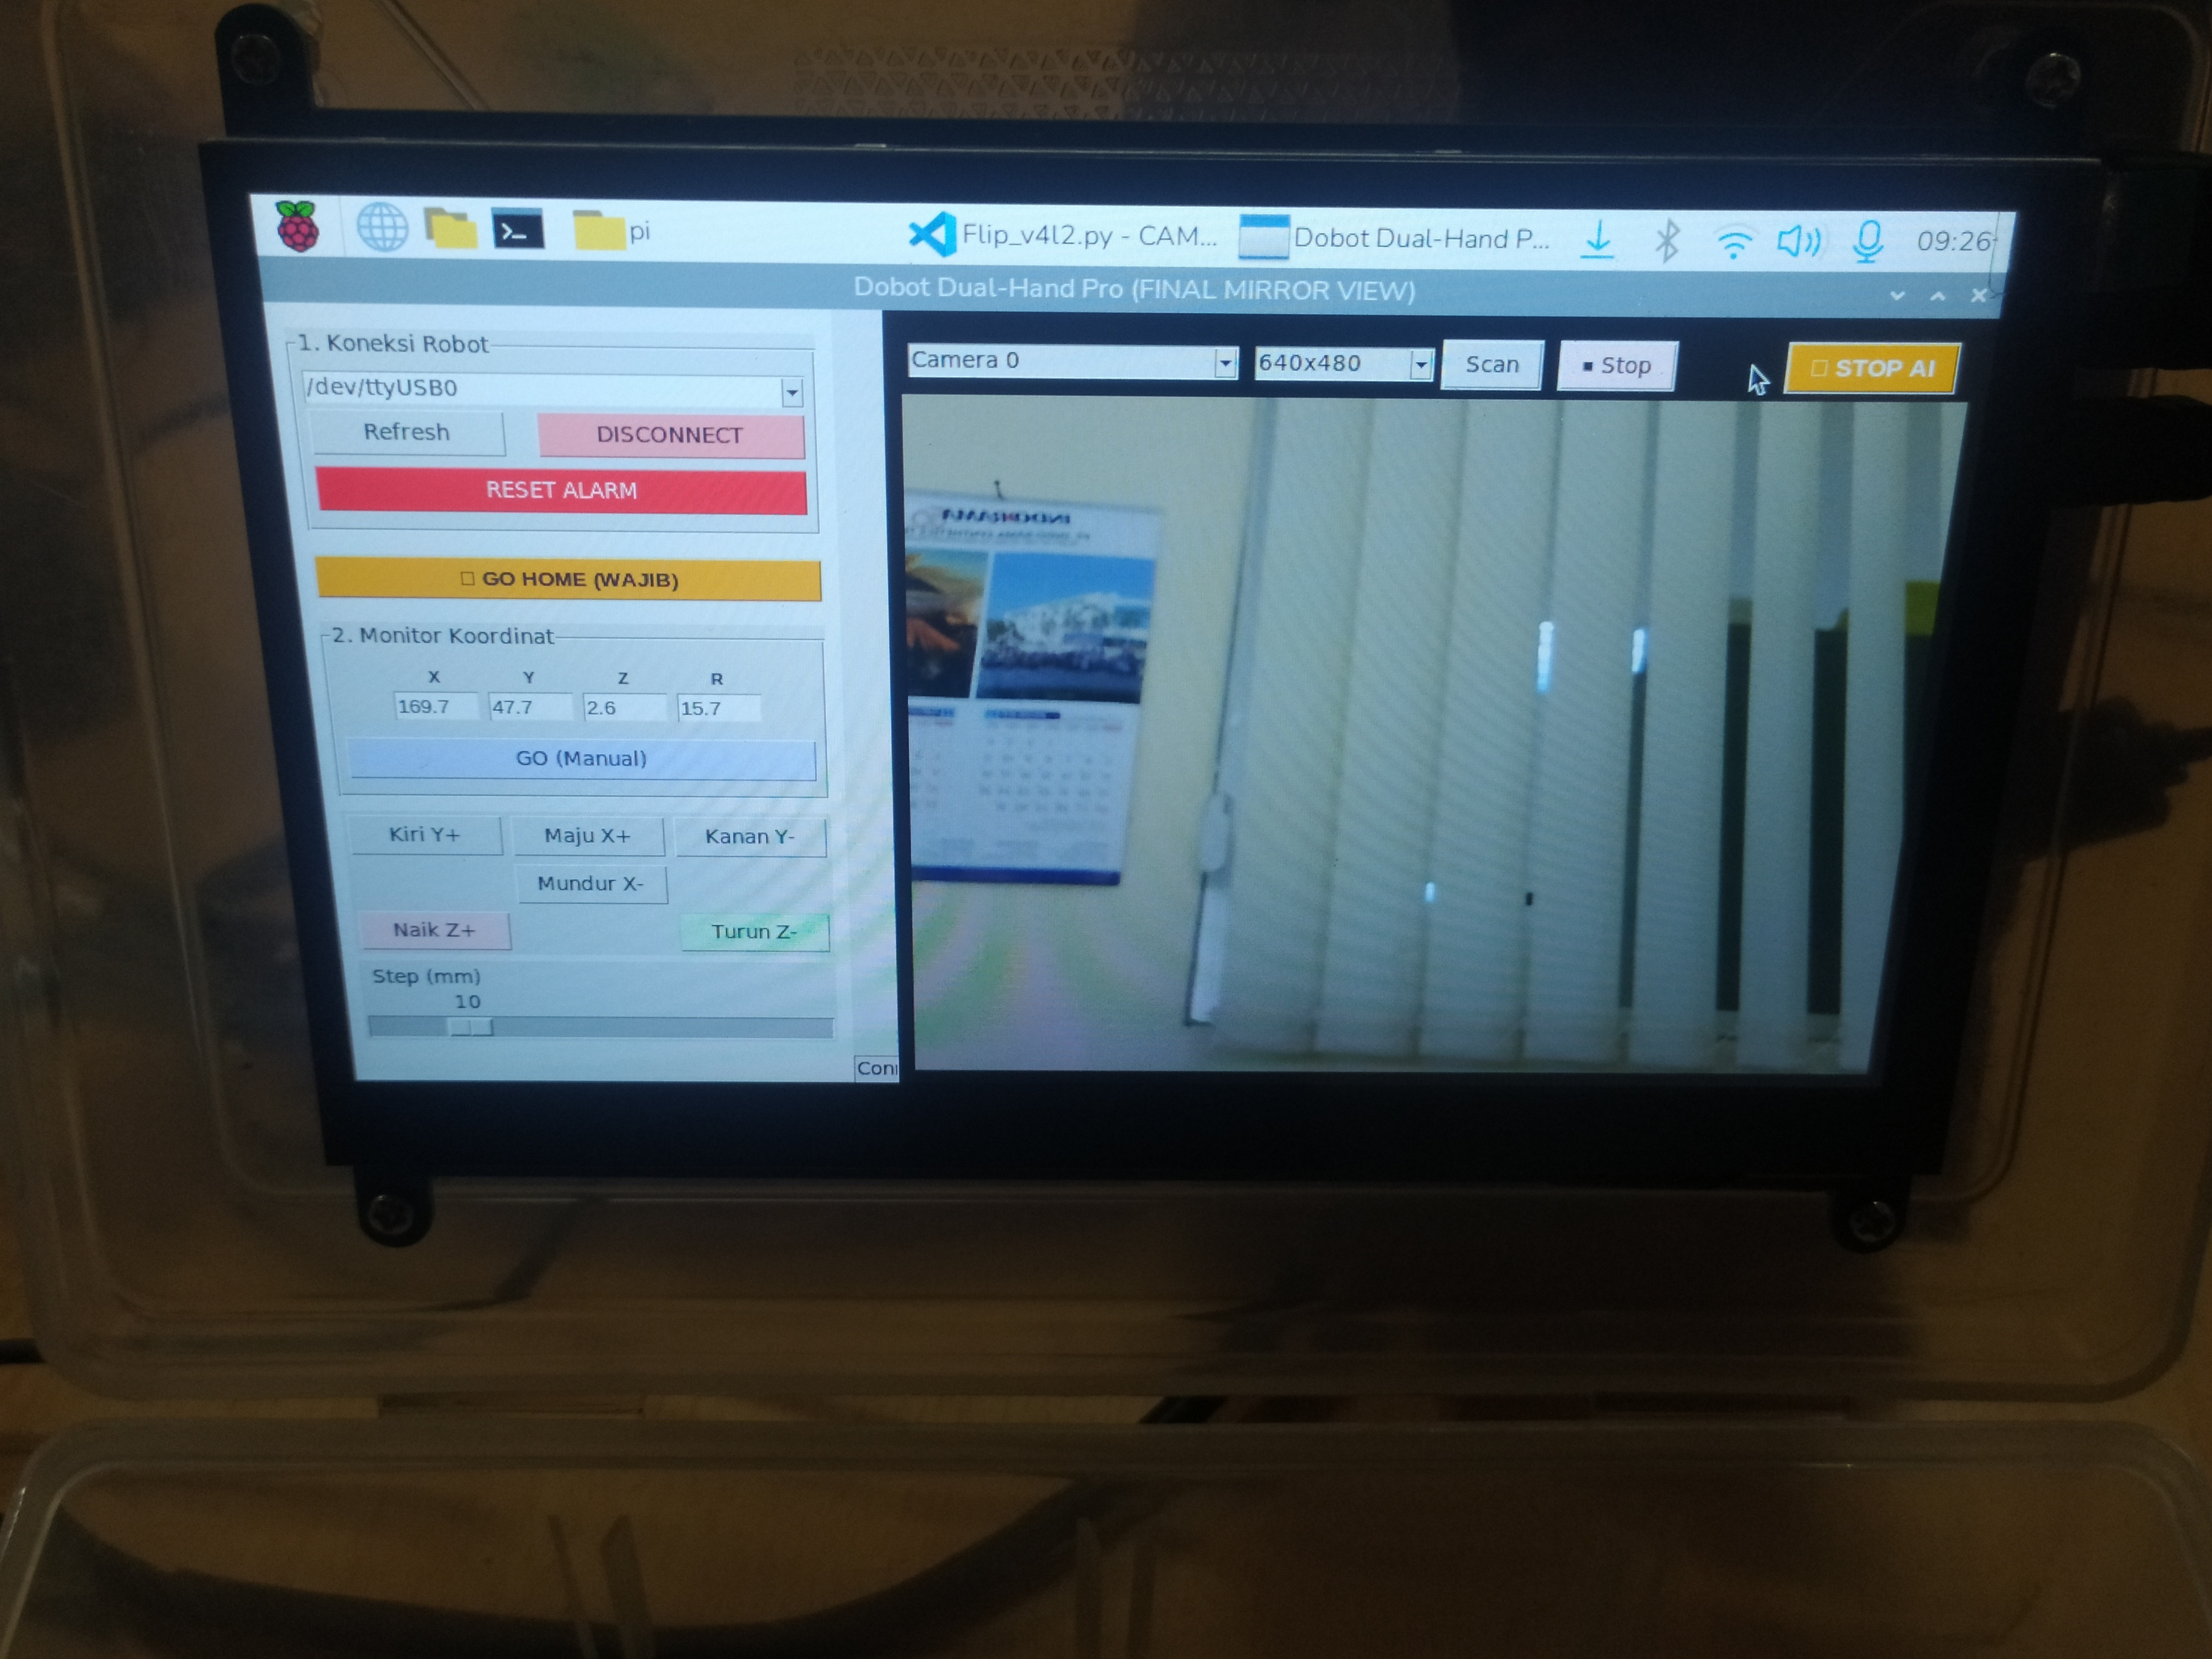
\includegraphics[width=0.85\textwidth]{Gambar/Gambar3_1_antarmuka_dobot.jpg}
    \caption{Antarmuka Sistem Visi Komputer Tertanam pada Kendali Dobot Magician}
    \label{fig:antarmuka_dobot}
\end{figure}

\section{Komputasi Tepi (\textit{Edge Computing}) dengan Raspberry Pi 5}
Komputasi tepi (\textit{edge computing}) adalah paradigma arsitektur teknologi informasi yang mendistribusikan beban kerja komputasi sedekat mungkin dengan sumber data sensorik \cite{satyanarayanan2017}. Dalam sistem robotika kendali visual, kamera bertindak sebagai node sensor berkecepatan tinggi yang terus menerus menghasilkan aliran data (\textit{data stream}). Jika aliran citra ini dikirim ke \textit{server} awan untuk diproses, akan terjadi disipasi \textit{bandwidth} yang besar dan latensi yang fluktuatif. Komputasi tepi menyelesaikan masalah ini dengan menarik kapabilitas analitik kecerdasan buatan langsung ke lapisan perangkat fisik (\textit{device layer}), memastikan waktu respons pergerakan robot berada pada batas waktu nyata (\textit{hard real-time constraints}).

Sebagai platform perangkat keras komputasi tepi, Raspberry Pi 5 ditenagai oleh \textit{System-on-Chip} (SoC) BCM2712 dengan arsitektur ARM Cortex-A76 \textit{quad-core} \cite{rpi5brief2023}. Peningkatan kinerja komputasi instruksi tunggal (\textit{single-thread}) pada mikrokontroler ini memungkinkannya untuk menjalankan model inferensi \textit{Deep Neural Networks} (DNN) dan pelacakan koordinat spasial tanpa memerlukan akselerator grafis terpisah (\textit{dedicated GPU}). Antarmuka PCIe 2.0 dan \textit{bandwidth} memori yang tinggi menjadikannya instrumen yang sangat mumpuni untuk purwarupa kendali robotika \textit{edge AI} berskala industri maupun edukasi \cite{wang2020}.

\section{Visi Komputer dan Ekstraksi Fitur Geometris (\textit{Landmark Extraction})}
Dalam sistem interaksi manusia-robot, proses pengolahan visual sering kali terkendala oleh besarnya beban komputasi apabila mengandalkan pemrosesan matriks piksel mentah \cite{rautaray2015}. Konversi dari citra warna (RGB) tiga kanal beresolusi tinggi secara langsung membutuhkan spesifikasi memori dan \textit{clock speed} yang jauh melampaui kapasitas rata-rata \textit{Single Board Computer} (SBC). Oleh karena itu, pendekatan ekstraksi fitur yang optimal untuk komputasi tepi harus beralih dari analisis piksel masif menuju pemahaman geometri struktur objek utama di dalam \textit{frame}.

Sebagai solusi efisiensi komputasi tepi, proses ekstraksi fitur difokuskan pada geometri struktur objek melalui metode \textit{landmark extraction} \cite{zhang2020}. Pada pendekatan ini, citra kasar tidak diklasifikasikan secara utuh, melainkan direduksi terlebih dahulu menjadi susunan titik-titik koordinat spasial yang merepresentasikan persendian kerangka objek (tangan). Kumpulan titik ini membentuk vektor numerik satu dimensi (1D array) yang sangat ringan. Vektor fitur spasial yang padat (\textit{dense feature vector}) inilah yang kemudian diumpankan maju (\textit{feed-forward}) ke dalam model \textit{Deep Neural Networks} (DNN) \textit{fully-connected} standar, memastikan \textit{inference time} dalam hitungan milidetik.

\section{Pengenalan Sistem Isyarat Bahasa Indonesia (SIBI) Berbasis DNN}
Sistem Isyarat Bahasa Indonesia (SIBI) merupakan tata bahasa isyarat formal yang memanfaatkan artikulasi jari-jemari tangan (\textit{dactylology}) dan posisi spasial tangan relatif terhadap tubuh untuk merepresentasikan abjad alfabet (A--Z) dan struktur numerik \cite{kosasih2012}. Setiap huruf dalam SIBI memiliki karakteristik lekukan jari dan orientasi telapak tangan yang sangat spesifik. Dalam konteks \textit{Human-Machine Interface} (HMI), variabilitas gestur ini merupakan kandidat ideal untuk digunakan sebagai pustaka instruksi mandiri (\textit{command library}), di mana setiap abjad dapat dipetakan secara eksklusif (\textit{one-to-one mapping}) pada aksi lengan robot meArm, seperti perintah buka-tutup \textit{gripper} atau transisi antar sumbu koordinat.

Dalam implementasi kendali ini, pengenalan abjad SIBI tidak menggunakan \textit{Convolutional Neural Networks} (CNN), melainkan diproses menggunakan arsitektur \textit{Deep Neural Networks} (DNN) standar \cite{goodfellow2016}. Fitur \textit{input} yang digunakan adalah nilai jarak relatif atau koordinat $(x,y,z)$ dari 21 titik persendian tangan hasil ekstraksi struktur geometris. Variasi kelengkungan jari pada formasi isyarat SIBI akan menghasilkan larik (\textit{array}) angka yang unik. DNN bertugas memodelkan probabilitas matematika dari susunan angka tersebut melalui fungsi aktivasi non-linear pada lapisan tersembunyi (\textit{hidden layers}). \textit{Output} dari lapisan akhir sistem DNN memprediksi probabilitas tertinggi dari formasi tangan untuk diklasifikasikan ke dalam instruksi spesifik (\textit{discrete control}).

\section{Pelacakan Gerak Tangan (\textit{Hand Tracking}) Menggunakan MediaPipe}
MediaPipe adalah kerangka kerja (\textit{framework}) lintas platform sumber terbuka yang dirancang oleh Google untuk membangun saluran inferensi (\textit{perception pipelines}) berbasis video dengan latensi sangat rendah \cite{lugaresi2019}. Keunggulan utama MediaPipe terletak pada kemampuannya untuk merangkai beberapa model \textit{Machine Learning} secara berurutan dalam sebuah \textit{graph} sinkron, memungkinkan eksekusi deteksi objek dinamis pada \textit{hardware} dengan spesifikasi terbatas tanpa menyebabkan \textit{bottleneck} pemrosesan.

Modul \textit{MediaPipe Hand Tracking} beroperasi menggunakan arsitektur inferensi dua tahap (\textit{two-stage architecture}) \cite{zhang2020}. Tahap pertama menggunakan algoritma detektor telapak tangan (\textit{palm detector model}) untuk melokalisasi \textit{bounding box} area tangan pada \textit{frame} gambar awal. Setelah tangan terlacak, tahap kedua menjalankan model penanda fitur (\textit{hand landmark model}) hanya pada area terpotong (\textit{cropped area}) tersebut untuk memprediksi 21 titik koordinat persendian spasial 3D $(x,y,z)$ secara presisi dan kontinu. Pendekatan prediksi berjenjang ini secara masif mereduksi beban komputasi. Koordinat inilah yang diekstrak sebagai \textit{input} larik numerik (\textit{array}) untuk model DNN pada mode pengenalan SIBI, serta digunakan sebagai target perpindahan sumbu spasial langsung pada mode teleoperasi dinamis Dobot Magician.

Topologi persebaran dan penamaan dari ke-21 titik persendian tangan tersebut diilustrasikan pada Gambar \ref{fig:mediapipe_landmarks}.

\begin{figure}[htbp]
    \centering
    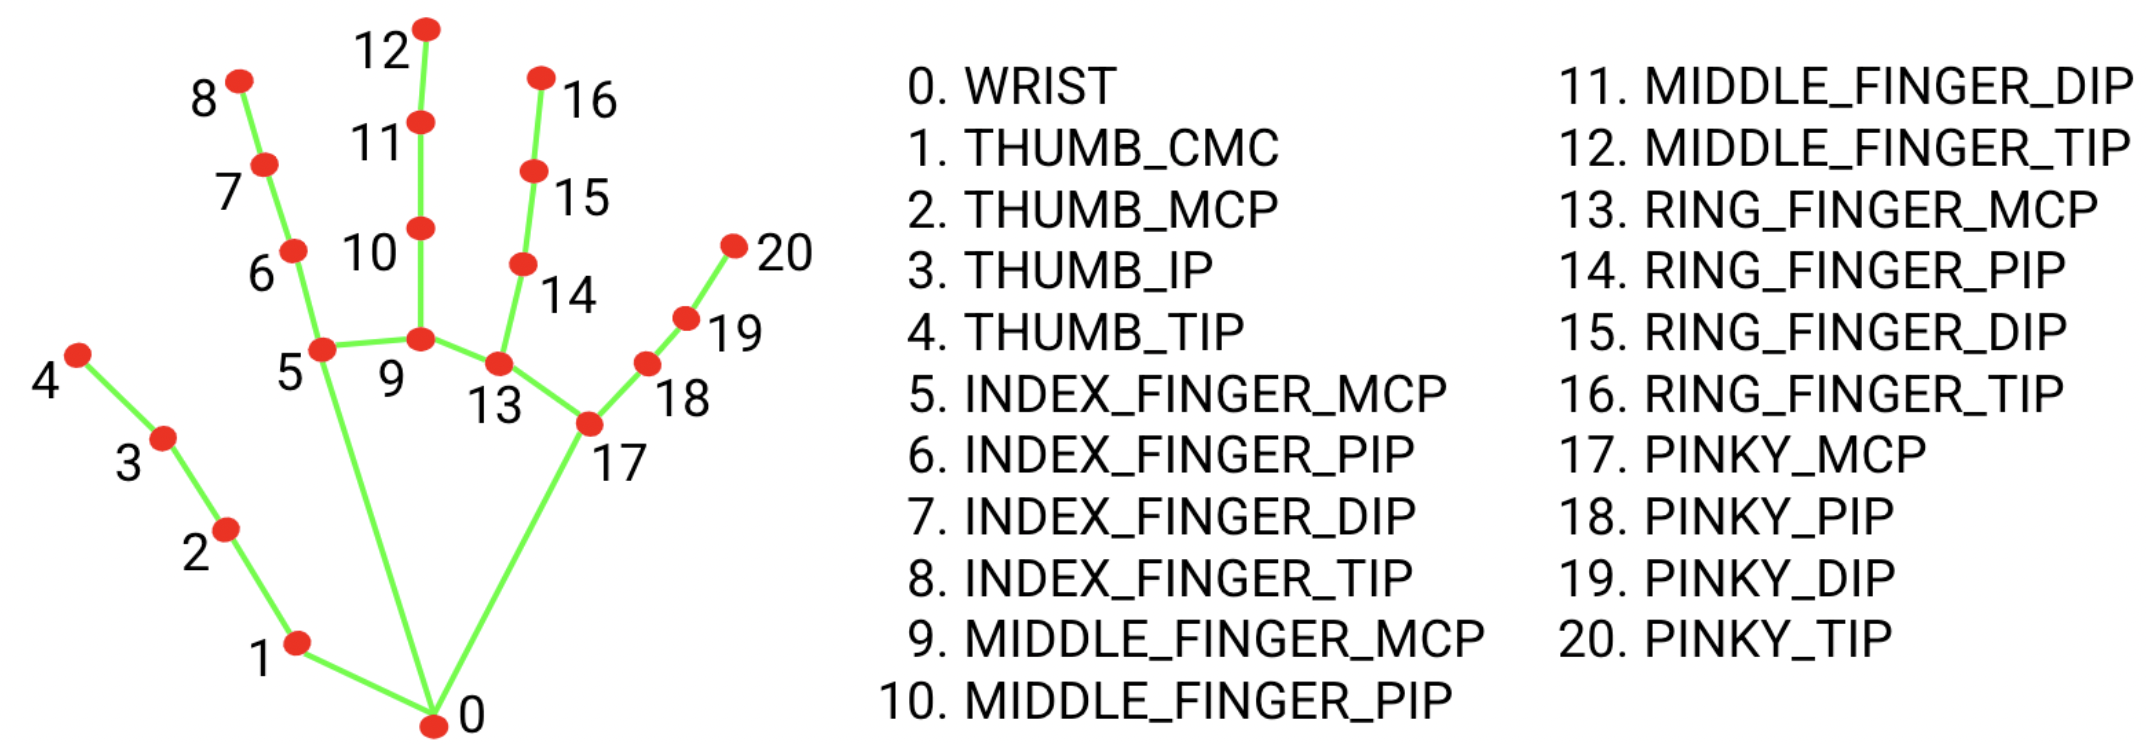
\includegraphics[width=0.85\textwidth]{Gambar/Gambar3_2_mediapipe_landmarks.png}
    \caption{Representasi 21 Titik Persendian Tangan (\textit{Hand Landmarks}) pada Framework MediaPipe}
    \label{fig:mediapipe_landmarks}
\end{figure}

Berdasarkan Gambar \ref{fig:mediapipe_landmarks}, setiap titik persendian tangan memiliki indeks anatomi spesifik, dimulai dari titik 0 yang merepresentasikan pergelangan tangan (WRIST). Titik pergelangan ini difungsikan sebagai titik acuan referensi origin $(0,0,0)$ dalam tahap normalisasi posisi spasial tangan. Titik persendian berikutnya terbagi ke dalam lima jari: ibu jari (titik 1--4: THUMB\_CMC, THUMB\_MCP, THUMB\_IP, THUMB\_TIP), jari telunjuk (titik 5--8: INDEX\_FINGER\_MCP hingga INDEX\_FINGER\_TIP), jari tengah (titik 9--12: MIDDLE\_FINGER\_MCP hingga MIDDLE\_FINGER\_TIP), jari manis (titik 13--16: RING\_FINGER\_MCP hingga RING\_FINGER\_TIP), dan kelingking (titik 17--20: PINKY\_MCP hingga PINKY\_TIP). Informasi spasial tiga dimensi $(x,y,z)$ dari seluruh titik persendian menghasilkan 63 nilai skalar fitur geometris yang merepresentasikan postur tangan secara invarian terhadap latar belakang visual.

\section{Kinematika Lengan Robot Manipulator 4-DOF}
Kinematika adalah cabang mekanika analitik yang mempelajari pergerakan murni suatu sistem benda multi-bodi tanpa mempertimbangkan gaya (torsi) maupun massa yang menyebabkan pergerakan tersebut \cite{craig2018}. Pada analisis lengan robot 4-DOF (\textit{Degree of Freedom}), sistem mekanis dimodelkan sebagai rangkaian segmen kaku (\textit{rigid links}) yang terhubung oleh persendian rotasional. Konfigurasi 4-DOF umumnya menyediakan tiga derajat kebebasan untuk translasi posisi pada koordinat spasial $(X,Y,Z)$ dan satu derajat kebebasan tambahan untuk mengontrol orientasi (\textit{pitch} sudut kemiringan) pada ujung efektor (\textit{end-effector}).

Penyelesaian matematis pergerakan ini sangat esensial dalam perancangan kendali robot dan terbagi menjadi dua penyelesaian utama, yaitu kinematika maju (\textit{forward kinematics}) dan kinematika balikan (\textit{inverse kinematics}) \cite{lynch2017}.

\subsection{Kinematika Maju (\textit{Forward Kinematics})}
Kinematika maju digunakan untuk menghitung posisi dan orientasi absolut dari \textit{end-effector} di ruang Cartesian berdasarkan besaran sudut rotasi yang diumpankan pada masing-masing motor sendi $(\theta_1, \theta_2, \theta_3, \theta_4)$. Berdasarkan pendekatan analisis geometris pada lengan robot artikulasi 4-DOF, lengan direpresentasikan dengan panjang tautan lengan atas ($L_1$), lengan bawah ($L_2$), dan tautan efektor ($L_3$). Tinggi basis dari titik tumpu dinyatakan sebagai $d_1$.

Orientasi sudut kemiringan (\textit{pitch angle}) dari \textit{end-effector} terhadap bidang horizontal disimbolkan dengan $\phi$, yang merupakan akumulasi dari rotasi sendi kedua hingga keempat:
\begin{equation}
\phi = \theta_2 + \theta_3 + \theta_4
\label{eq:phi}
\end{equation}

Posisi radius jangkauan horizontal ($r$) pada bidang proyeksi dua dimensi dirumuskan melalui penjumlahan vektor trigonometri berikut:
\begin{equation}
r = L_1 \cos(\theta_2) + L_2 \cos(\theta_2 + \theta_3) + L_3 \cos(\phi)
\label{eq:r}
\end{equation}

Berdasarkan nilai radius tersebut, proyeksi koordinat Cartesian spasial $(X,Y,Z)$ untuk posisi akhir ujung robot dapat dikalkulasi secara lengkap menggunakan himpunan persamaan:
\begin{equation}
\begin{cases}
X = r \cos(\theta_1), \\
Y = r \sin(\theta_1), \\
Z = d_1 + L_1 \sin(\theta_2) + L_2 \sin(\theta_2 + \theta_3) + L_3 \sin(\phi).
\end{cases}
\label{eq:fk}
\end{equation}
di mana $\theta_1$ mewakili sudut putar pada sendi basis (\textit{base yaw}).

\subsection{Kinematika Balikan (\textit{Inverse Kinematics})}
Kinematika balikan merupakan proses komputasi untuk mencari nilai sudut persendian $(\theta_1, \theta_2, \theta_3, \theta_4)$ yang dibutuhkan agar \textit{end-effector} mencapai target koordinat spasial $(X,Y,Z)$ dengan sudut orientasi $\phi$ tertentu \cite{craig2018}. Penyelesaian pada robot 4-DOF diuraikan dalam beberapa tahapan komputasi geometris.

Pertama, sudut putar basis ($\theta_1$) dan jarak radius planar ($r$) dihitung menggunakan fungsi tangen dua argumen dan teorema Pythagoras:
\begin{equation}
\begin{cases}
\theta_1 = \text{atan2}(Y, X), \\
r = \sqrt{X^2 + Y^2}.
\end{cases}
\label{eq:ik_theta1}
\end{equation}

Tahap kedua adalah mendekomposisi posisi \textit{end-effector} untuk menemukan koordinat persendian pergelangan atau \textit{wrist center} $(r_w, z_w)$. Titik ini merupakan ujung dari tautan $L_2$ dan pangkal dari $L_3$:
\begin{equation}
\begin{cases}
r_w = r - L_3 \cos(\phi), \\
z_w = Z - d_1 - L_3 \sin(\phi).
\end{cases}
\label{eq:wrist_center}
\end{equation}

Tahap ketiga menerapkan Hukum Kosinus pada segitiga yang dibentuk oleh $L_1$, $L_2$, dan garis hipotenusa imajiner yang menghubungkan pangkal $L_1$ dengan \textit{wrist center}. Sudut sendi siku ($\theta_3$) diselesaikan dengan persamaan:
\begin{equation}
\begin{cases}
c_3 = \dfrac{r_w^2 + z_w^2 - L_1^2 - L_2^2}{2 L_1 L_2}, \\[10pt]
\theta_3 = \text{atan2}\left(\pm \sqrt{1 - c_3^2}, c_3\right).
\end{cases}
\label{eq:ik_theta3}
\end{equation}
dengan $c_3 = \cos(\theta_3)$. Tanda $\pm$ mengindikasikan keberadaan dua solusi postur (\textit{elbow-up} atau \textit{elbow-down}).

Tahap keempat menghitung sudut sendi bahu ($\theta_2$) dengan memanfaatkan sudut dekomposisi $\alpha$ dan $\beta$:
\begin{equation}
\begin{cases}
\alpha = \text{atan2}(z_w, r_w), \\[6pt]
\beta = \text{atan2}(L_2 \sin(\theta_3), L_1 + L_2 \cos(\theta_3)), \\[6pt]
\theta_2 = \alpha - \beta.
\end{cases}
\label{eq:ik_theta2}
\end{equation}

Tahap terakhir adalah mengkalkulasi sudut sendi pergelangan ($\theta_4$) berdasarkan nilai orientasi $\phi$ yang telah ditetapkan:
\begin{equation}
\theta_4 = \phi - \theta_2 - \theta_3
\label{eq:ik_theta4}
\end{equation}

\subsection{Implementasi pada Perangkat Keras 4-DOF}
Pemodelan matematis ini diimplementasikan secara spesifik pada dua varian lengan robot 4-DOF:

\subsubsection{Dobot Magician}
Dobot Magician merupakan lengan robot industrial yang digerakkan menggunakan aktuator motor \textit{stepper} berpresisi tinggi \cite{dobot2022, dobot2026}. Kestabilan mekanisnya sangat ideal untuk mode teleoperasi dinamis, sebagaimana ditunjukkan pada Gambar \ref{fig:dobot_magician}. Pada mode ini, penyelesaian \textit{inverse kinematics} (Persamaan (\ref{eq:ik_theta1}) hingga Persamaan (\ref{eq:ik_theta4})) dieksekusi secara kontinu oleh Raspberry Pi untuk mengonversi pergeseran matriks $(x,y,z)$ dari \textit{landmark} tangan manusia menjadi matriks sudut $(\theta_1, \theta_2, \theta_3, \theta_4)$. Data sudut ini kemudian ditransmisikan ke pengendali internal robot agar mampu mereplikasi pergerakan tangan operator secara \textit{real-time}.

\begin{figure}[htbp]
    \centering
    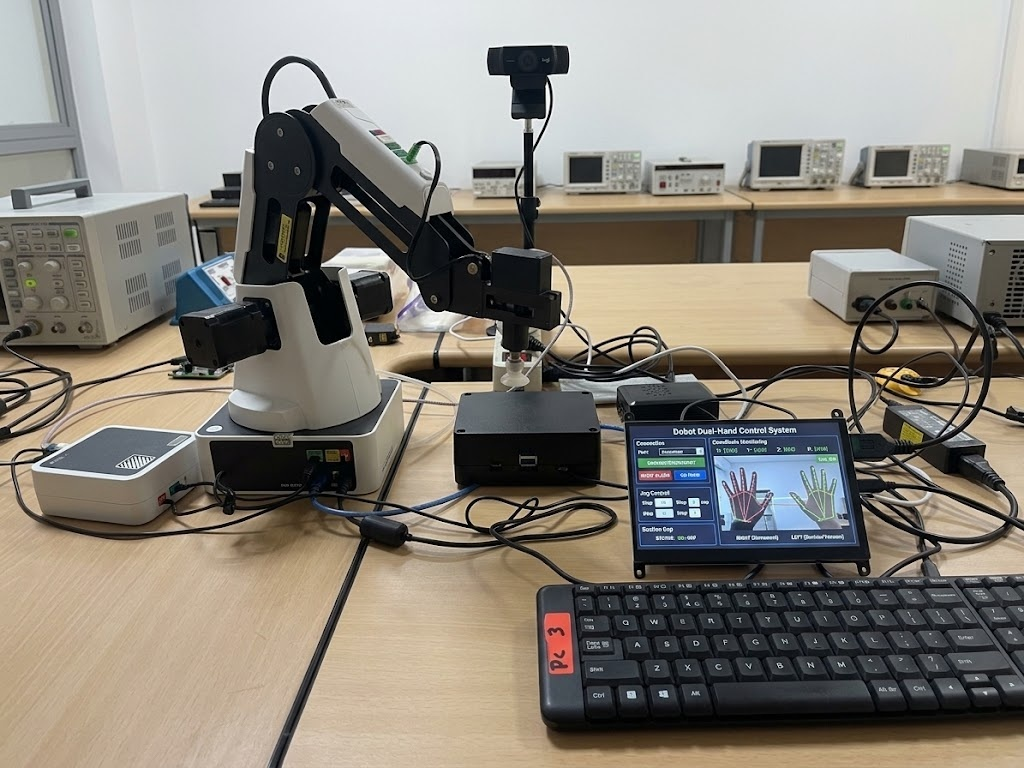
\includegraphics[width=0.75\textwidth]{Gambar/Gambar3_3_dobot_magician.jpg}
    \caption{Lengan Robot Dobot Magician untuk Implementasi Teleoperasi Dinamis}
    \label{fig:dobot_magician}
\end{figure}

\subsubsection{meArm}
meArm adalah purwarupa manipulator berskala kecil berbahan dasar akrilik yang digerakkan oleh motor servo standar \cite{mearm2026}. Konfigurasi fisik purwarupa meArm tampak depan dan tampak samping diilustrasikan pada Gambar \ref{fig:mearm_prototype}. Konfigurasi mekanis ini digunakan secara khusus untuk mode kendali diskret berbasis pengenalan SIBI. Pergerakan meArm difokuskan pada perpindahan absolut dari posisi \textit{home} menuju koordinat kerja yang telah diprogram untuk menjepit atau memindahkan objek setelah isyarat SIBI terdeteksi secara valid.

\begin{figure}[htbp]
    \centering
    \begin{subfigure}[b]{0.48\textwidth}
        \centering
        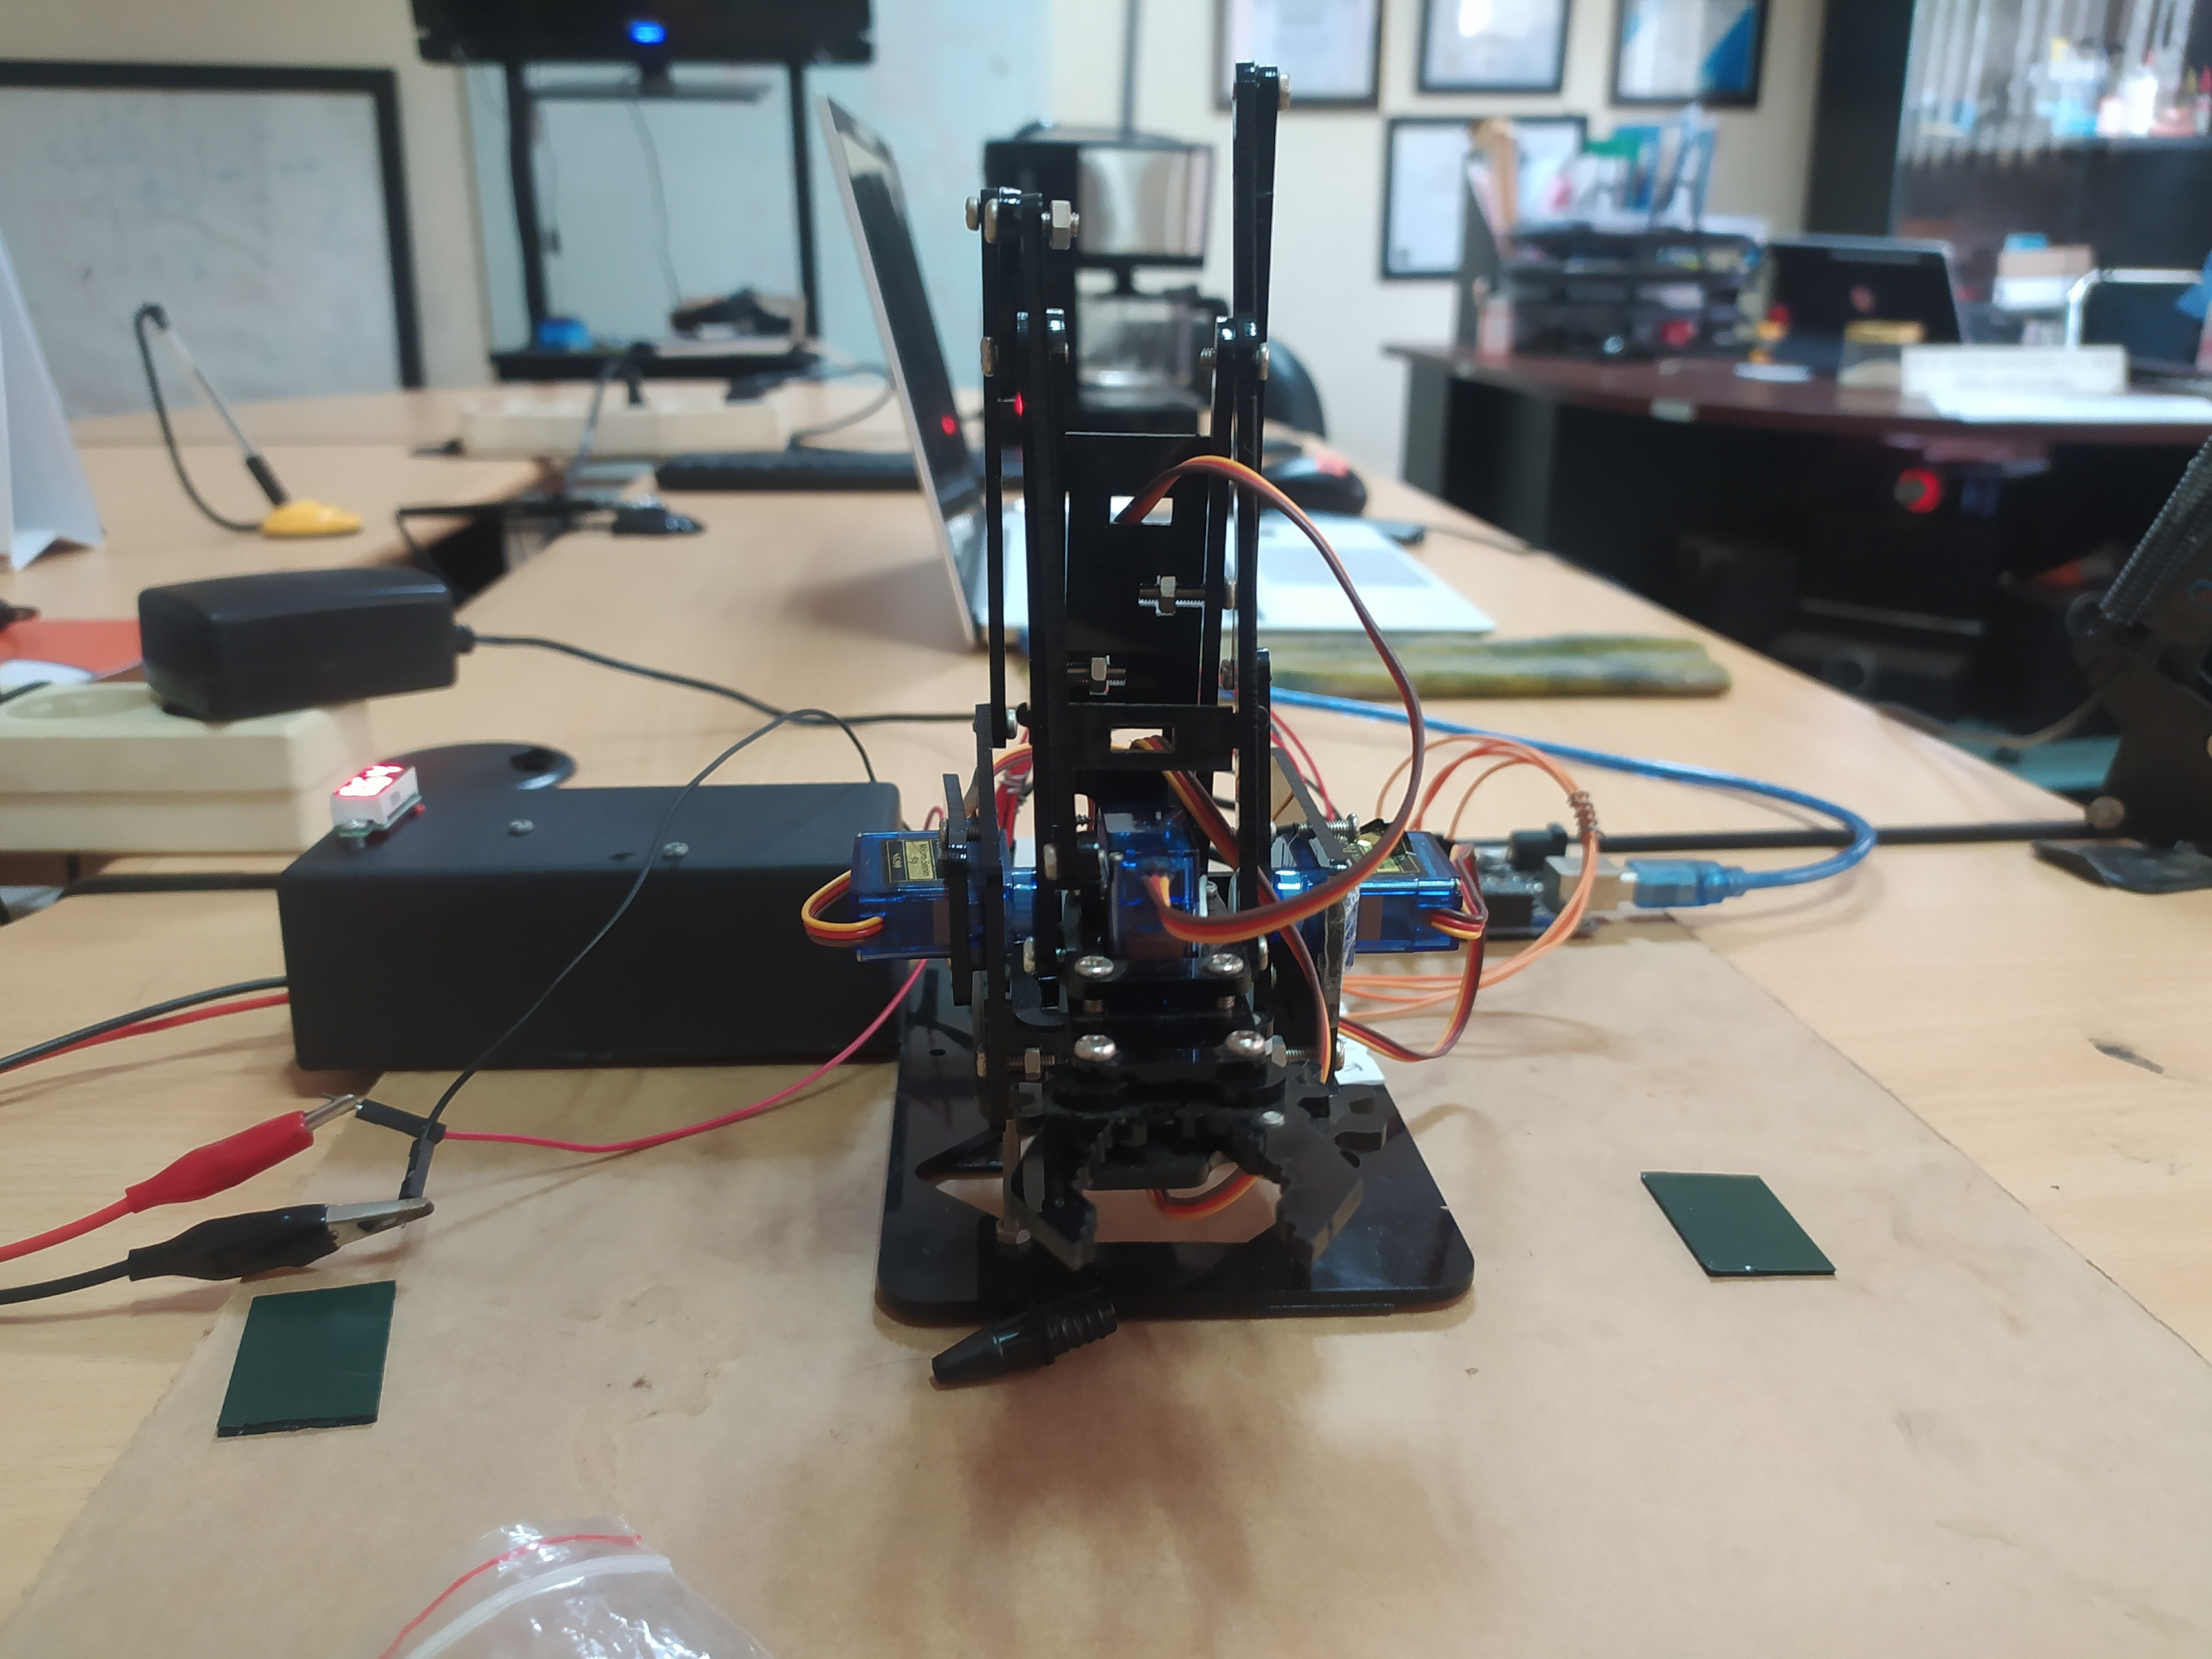
\includegraphics[width=\textwidth]{Gambar/Gambar3_4a_mearm_depan.jpg}
        \caption{Tampak Depan}
        \label{fig:mearm_depan}
    \end{subfigure}
    \hfill
    \begin{subfigure}[b]{0.48\textwidth}
        \centering
        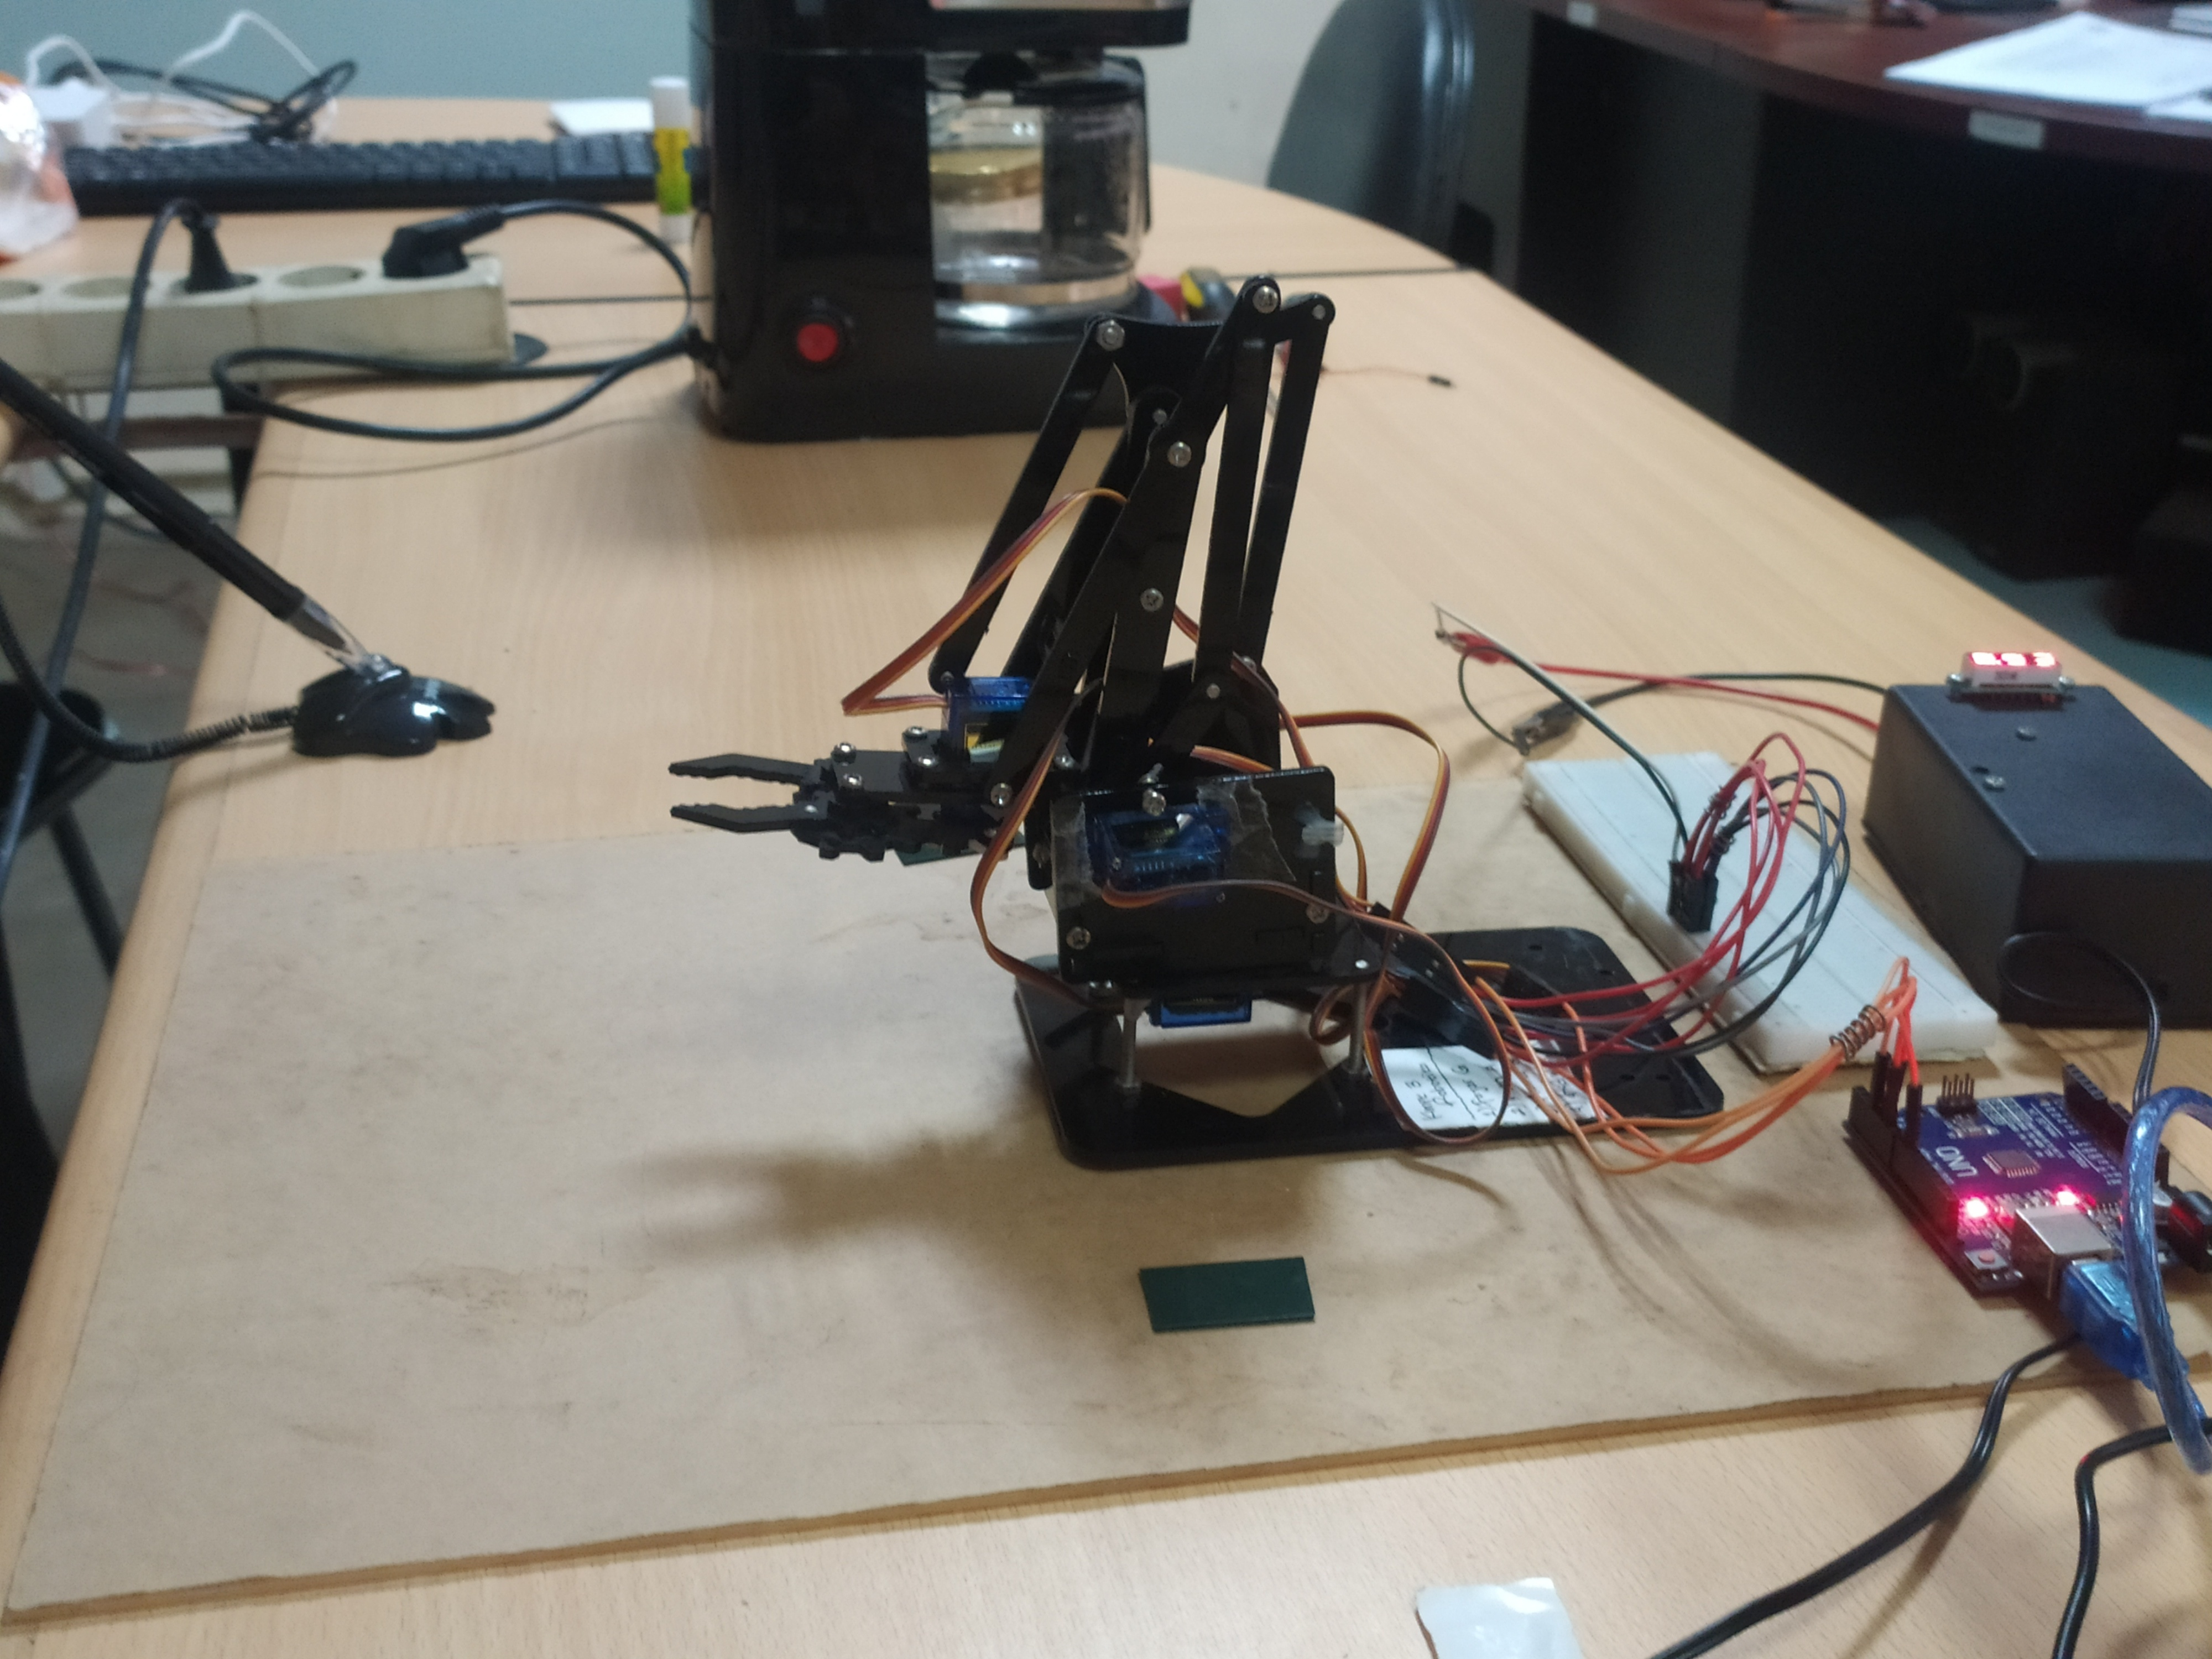
\includegraphics[width=\textwidth]{Gambar/Gambar3_4b_mearm_samping.jpg}
        \caption{Tampak Samping}
        \label{fig:mearm_samping}
    \end{subfigure}
    \caption{Purwarupa Lengan Robot meArm 4-DOF: (a) Tampak Depan dan (b) Tampak Samping untuk Mode Pengenalan SIBI}
    \label{fig:mearm_prototype}
\end{figure}

\section{Python 3.9}
Python 3.9 digunakan sebagai bahasa pemrograman utama karena memiliki sintaks yang ringkas, dukungan pustaka yang luas, serta kompatibilitas dengan banyak modul visi komputer dan komunikasi perangkat keras. Python 3.9 dirilis dengan berbagai penyempurnaan bahasa dan pustaka standar \cite{python39}. Pada penelitian ini, Python digunakan untuk membaca kamera, menjalankan MediaPipe, mengolah \textit{landmark} tangan, melakukan klasifikasi sederhana, mengirim perintah ke robot, serta mencatat data pengujian.

Selain Python, pustaka seperti NumPy dapat digunakan untuk operasi matriks dan pengolahan \textit{array} numerik \cite{harris2020}. Hal ini penting karena pemetaan koordinat, normalisasi fitur, dan perhitungan kinematika membutuhkan operasi vektor dan matriks yang efisien.
